\documentclass[11pt,spanish]{article} % Tipo y tamaño de letra del documento.


\usepackage[utf8]{inputenc}
\usepackage{subfiles}
\usepackage{biblatex}
\addbibresource{references.bib}
\usepackage{multicol}
\usepackage{amsfonts}
\usepackage{blindtext}
\usepackage{mathrsfs}
\usepackage{amsmath}
\usepackage{siunitx}
\usepackage{centernot}
\usepackage[shortlabels]{enumitem}
\usepackage{subfig}
\usepackage{datetime}
\usepackage{listingsutf8}
\usepackage[spanish]{babel}
\usepackage{tikz}
\usepackage{hyperref}
\usepackage[vlined,ruled,linesnumbered]{algorithm2e}
\usepackage{listings}
\usepackage{float}
\usepackage{url}
\usepackage{csquotes}
\usepackage{fourier} %font
\usepackage[top=2cm, bottom=2cm, left=2.5cm, right=2.5cm]{geometry}
\usepackage{pgfplots}
\usepackage{fancyhdr}
\usepackage{mdframed}
\usepackage{tikzducks}
\usepackage[nameinlink]{cleveref}
\usepackage{epigraph} 

\pgfplotsset{compat=1.18}

\usetikzlibrary{shapes.arrows, shapes.geometric, arrows.meta,angles,quotes,positioning,arrows,fit,quotes,calc}
\tikzset{>=latex} 

\setlength\algomargin{1em} 
\SetFuncSty{sc} 
\SetCommentSty{em} 


\Crefname{figure}{Fig.}{Figs.}
\newcommand\crefrangeconjunction{--}
\Crefname{table}{Tabla}{Tablas}
\Crefname{subsubsection}{Subsubsec.}{Subsubsections}
\Crefname{subsection}{Subsec.}{Subsections}
\Crefname{section}{Sec.}{Sections}
\Crefname{equation}{eq.}{eqs.}
\crefname{thm}{Theorem}{theorems}
\Crefname{thm}{Theorem}{Theorems} 

\definecolor{algoco}{rgb}{0,0.0,1}

\hypersetup{
  colorlinks=true,
  linkcolor=algoco,
  citecolor=blue,
  urlcolor=blue,
}

\lstset{
extendedchars=true
inputencoding=utf8/latin1,
basicstyle=\footnotesize\sffamily\color{black},
commentstyle=\slshape \color{gray},
numbers=left,
numbersep=10pt,
numberstyle=\tiny\color{red!80!black},
keywordstyle=\color{red!80!magenta},
showspaces=false,
showstringspaces=false,
stringstyle=\color{cyan!80!black},
tabsize=2,
literate={á}{{\'a}}1 {é}{{\'e}}1 {í}{{\'i}}1 {ó}{{\'o}}1 {ú}{{\'u}}1,
frame = single, 
numbers = none,
float, floatplacement = ht, captionpos = b,
xleftmargin = 2em, xrightmargin = 2em, 
}

\newcommand{\ub}[1]{\underbrace{#1}}
\newcommand\tcm{\textbf}
\newcommand\tca{\textcolor{algoco}}

\setlength\epigraphwidth{.7\textwidth} 

\newcommand{\tnum}{1} % reemplace 1 por el número de la tarea
\newcommand{\sem}{2025-1} % reemplace 2024-2 por el semestre correspondiente
\newcommand{\campus}{Casa Central \\ Valparaíso} % reemplace Casa Central por el campus correspondiente
\newcommand{\rolusm}{202673100-1} % reemplace 2025073100-1 por su rol
\newcommand{\namestudent}{Al Goritmo Pérez} % reemplace Al Goritmo Pérez por su nombre
\newcommand{\deadline}{21 de abril de 2025 } % reemplace 26 de abril de 2025, medio día por la fecha de entrega

\headheight=14pt
\linespread{1.3}
\author{\namestudent}
\pagestyle{fancy}
\fancyhf{}%
\fancyfoot[R]{ \namestudent \\ \rolusm}
\fancyfoot[L]{Campus \campus} 
\fancyfoot[C]{\thepage}
\rhead{\sem}
\lhead{INF-221}
\renewcommand{\headrulewidth}{0.4pt}
\renewcommand{\footrulewidth}{0.4pt}
\newbool{programs}
\boolfalse{programs}
\chead{REPORTE TAREA \tnum~}



\title{
  \huge
  \textbf{REPORTE TAREA \tnum~ \\ ALGORITMOS Y COMPLEJIDAD} \\[1ex]
  \emph{\textquote{Más allá de la notación asintótica: Análisis experimental de algoritmos de ordenamiento y multiplicación de matrices.}} 
  }

  
\date{
  \small
  \today\\
  \currenttime
}




\begin{document}
\maketitle
\thispagestyle{fancy} 
\vspace{-1.0\baselineskip}




\begin{abstract}
  \textit{ 
    Este trabajo presenta un análisis experimental comparativo entre algoritmos de ordenamiento (SelectionSort, MergeSort y QuickSort) y de multiplicación de matrices (Naive y Strassen), evaluando la brecha entre su complejidad teórica y su rendimiento práctico. Implementados en C++, los algoritmos fueron sometidos a pruebas con conjuntos de datos de tamaños crecientes (hasta \(n = 10^7\) para ordenamiento y matrices de \(1024 \times 1024\)) y características variadas (aleatorios, ordenados, densos, diagonales y dispersos). Los resultados confirman que SelectionSort se vuelve inviable para \(n \geq 10^5\), mientras que los algoritmos de complejidad \(O(n \log n)\) mantienen eficiencia incluso con grandes volúmenes de datos, siendo \texttt{std::sort} el más rápido. Para la multiplicación de matrices, Strassen ofrece ventajas marginales solo en casos específicos (\(n \approx 256\)), pues la sobrecarga de recursión y gestión de memoria contrarresta sus beneficios teóricos en dimensiones mayores. Se concluye que la elección óptima de algoritmo depende no solo de su complejidad asintótica, sino también de las características del hardware y los patrones de datos, sugiriéndose la exploración de implementaciones híbridas para un alto rendimiento.
  }
     
\end{abstract}

\setcounter{tocdepth}{1}
\tableofcontents


\newpage
\section{Introducción}
\begin{mdframed}
    \textbf{La extensión máxima para esta sección es de 1 página.}
\end{mdframed}

La introducción de este tipo de informes o reportes, tiene como objetivo principal \textbf{contextualizar el problema que se va a analizar}, proporcionando al lector la información necesaria para entender la relevancia del mismo. 

Es fundamental que en esta sección se presenten los antecedentes del problema, destacando investigaciones previas o principios teóricos que sirvan como base para los análisis posteriores. Además, deben explicarse los objetivos del informe, que pueden incluir la evaluación de un algoritmo, la comparación de métodos o la validación de resultados experimentales.

Aunque la estructura y el enfoque siguen principios de trabajos académicos, se debe recordar que estos informes no son publicaciones científicas formales, sino trabajos de pregrado. Por lo tanto, se busca un enfoque claro y directo, que permita al lector comprender la naturaleza del problema y los objetivos del análisis, sin entrar en detalles excesivos. 


Introduction Checklist de \citetitle{GoodScientificPaper} \cite{GoodScientificPaper}, adaptada a nuestro contexto:

\begin{itemize}
\item Indique el \textbf{campo del trabajo} (Análisis y Diseño de algoritmos en Ciencias de la Computación), por qué este campo es importante y qué se ha hecho ya en este área, con las \textbf{citas} adecuadas de la literatura académica o fuentes relevantes.
\item Identifique una \textbf{brecha} en el conocimiento, un desafío práctico, o plantee una \textbf{pregunta} relacionada con la eficiencia, complejidad o aplicabilidad de un algoritmo particular.
\item Resuma el propósito del informe e introduzca el análisis o experimento, dejando claro qué se está investigando o comparando, e indique \textbf{qué es novedoso} o por qué es significativo en el contexto de un curso de pregrado.
\item Evite; repetir el resumen; proporcionar información innecesaria o fuera del alcance de la materia (limítese al análisis de algoritmos o conceptos de complejidad); exagerar la importancia del trabajo (recuerde que se trata de un informe de pregrado); afirmar novedad sin una comparación adecuada con lo enseñado en clase o la bibliografía recomendada.
\end{itemize}



\begin{mdframed}
Recuerde que este es su trabajo, y sólo usted puede expresar con precisión lo que ha aprendido y quiere transmitir. Si lo hace bien, su introducción será más significativa y valiosa que cualquier texto automatizado. ¡Confíe en sus habilidades, y verá que puede hacer un mejor trabajo que cualquier herramienta que automatiza la generación de texto!
\end{mdframed}



\newpage
\section{Implementaciones}
\begin{mdframed}
    \textbf{La extensión máxima para esta sección es de 1 página.}
\end{mdframed}


Sólo agregar la url del repositorio de GitHub donde se encuentra el código fuente de la tarea. Recordar que el repositorio \textbf{debe ser privado}, ya que de lo contrario cualquier persona podrá acceder a su código y cometer plagio, siendo usted responsable de ello. 

\begin{mdframed}
    \begin{center}
        {\Large \url{https://github.com/pabloealvarez/INF221-2025-1-TAREA-1}}
    \end{center}
\end{mdframed}




\newpage
\section{Experimentos}
Para asegurar la reproducibilidad de los experimentos y con el fin de que otros puedan verificar y extender estos resultados,se detalla a continuación la infraestructura utilizada.\\

El hardware consiste en:

- un procesador Apple M1,

- 8 GB de memoria RAM 

- almacenamiento en SSD NVMe.
\\

El entorno software corresponde a MacOS 15.4.1 Sequoia, compilador \texttt{c++17}, y las librerías estándar de C++ junto con el módulo \texttt{<chrono>} para la toma de tiempos. Todos los scripts de generación de datos y de gráficas fueron escritos en Python 3.8, empleando \texttt{matplotlib} y automatizados mediante un \texttt{Makefile}.

\subsection{Dataset (casos de prueba)}
Los casos de prueba empleados en este informe fueron los proporcionados en el enunciado, generados por los scripts en Python entregados originalmente. No se consideraron tamaños de entrada adicionales ni variaciones externas. Los conjuntos cubren:
\begin{itemize}
  \item \textbf{Ordenamiento:}
  \\
    - Tipo de datos: Los datos de los archivos de prueba estan conformados por solo numeros enteros.
    
    - Tamaño de la muestra: Los tamanios de muestra abarcan  $n = {10; 1000; 100000; 10 000 000}$, con distintos largo de los numeros siendo de 1 a 7 dígitos.
    
    - Distribución: ascendente, descendente y aleatoria, cada una con 3 casos por cada tamaño y distribución de los datos
    
    - Método de generación: Todos y cada uno de los casos de prueba se generan con el script presente en \path{/code/sorting/scripts/array_generator.py}


    


  \item \textbf{Multiplicación de matrices:}
    \\
    - Tipo de datos: Los datos de los archivos de prueba estan conformados por solo numeros enteros.
    
    - Tamaño de la muestra: Los tamaños de muestra abarcan  $n = {16,64,256,1024}$, con distintos tipos de números, pudiendo los valores ser binarios (0 y 1) o Decimales (0 al 9).
    
    - Distribución: Matices Densas, Diagonales y Dispersas, cada una con 3 casos por cada tamaño y distribución de los datos
    
    - Método de generación: Todos y cada uno de los casos de prueba se generan automaticamente con el script presente en \path{code/matrix_multiplication/scripts/matrix_generator.py}    
  
   
\end{itemize}



\subsection{Resultados}
\begin{mdframed}
    \textbf{La extensión máxima para esta sección es de 6 páginas.}
\end{mdframed}


En esta sección, los resultados obtenidos, como las gráficas o tablas, deben estar respaldados por los datos generados durante la ejecución de sus programas. Es fundamental que, junto con el informe, se adjunten los archivos que contienen dichos datos para permitir su verificación. Además, se debe permitir y especficiar como obtener esos archivos desde una ejecución en otro computador (otra infraestructura para hacer lso experimentos).

\textbf{Es necesario automatizar la generación de las gráficas}, ya que es imprescindible que se pueda confirmar que las visualizaciones presentadas son producto de los datos generados por sus algoritmos.

Agregue gráficas que muestren los resultados de sus experimentos. La cantidad de páginas es limitada, por lo tanto escoja las gráficas más representativas y que muestren de manera clara los resultados obtenidos. Esta elección es parte de lo que se evaluara en la sección de presentación de resultados. Referencie las figuras en el texto, describa lo que se observa en ellas y por qué son relevantes.




\begin{figure}[H]
    \centering
    \begin{minipage}[t]{0.5\textwidth}
        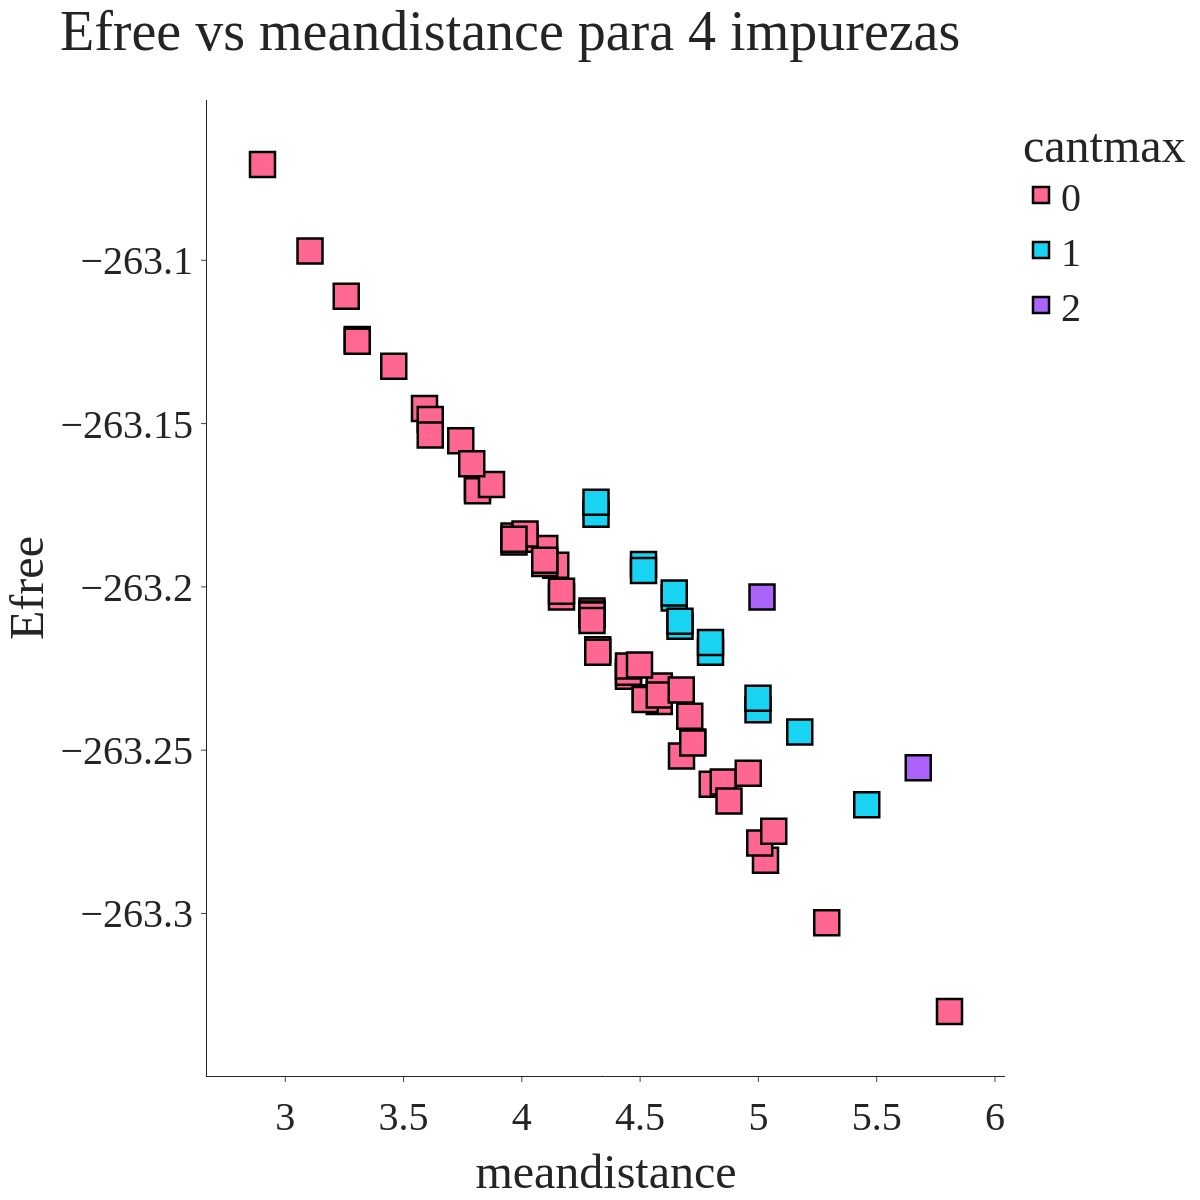
\includegraphics[width=\textwidth]{../code/matrix_multiplication/data/plots/4_impurezas_cantmax_size10.png}
    \end{minipage}%
    \begin{minipage}[t]{0.5\textwidth}
        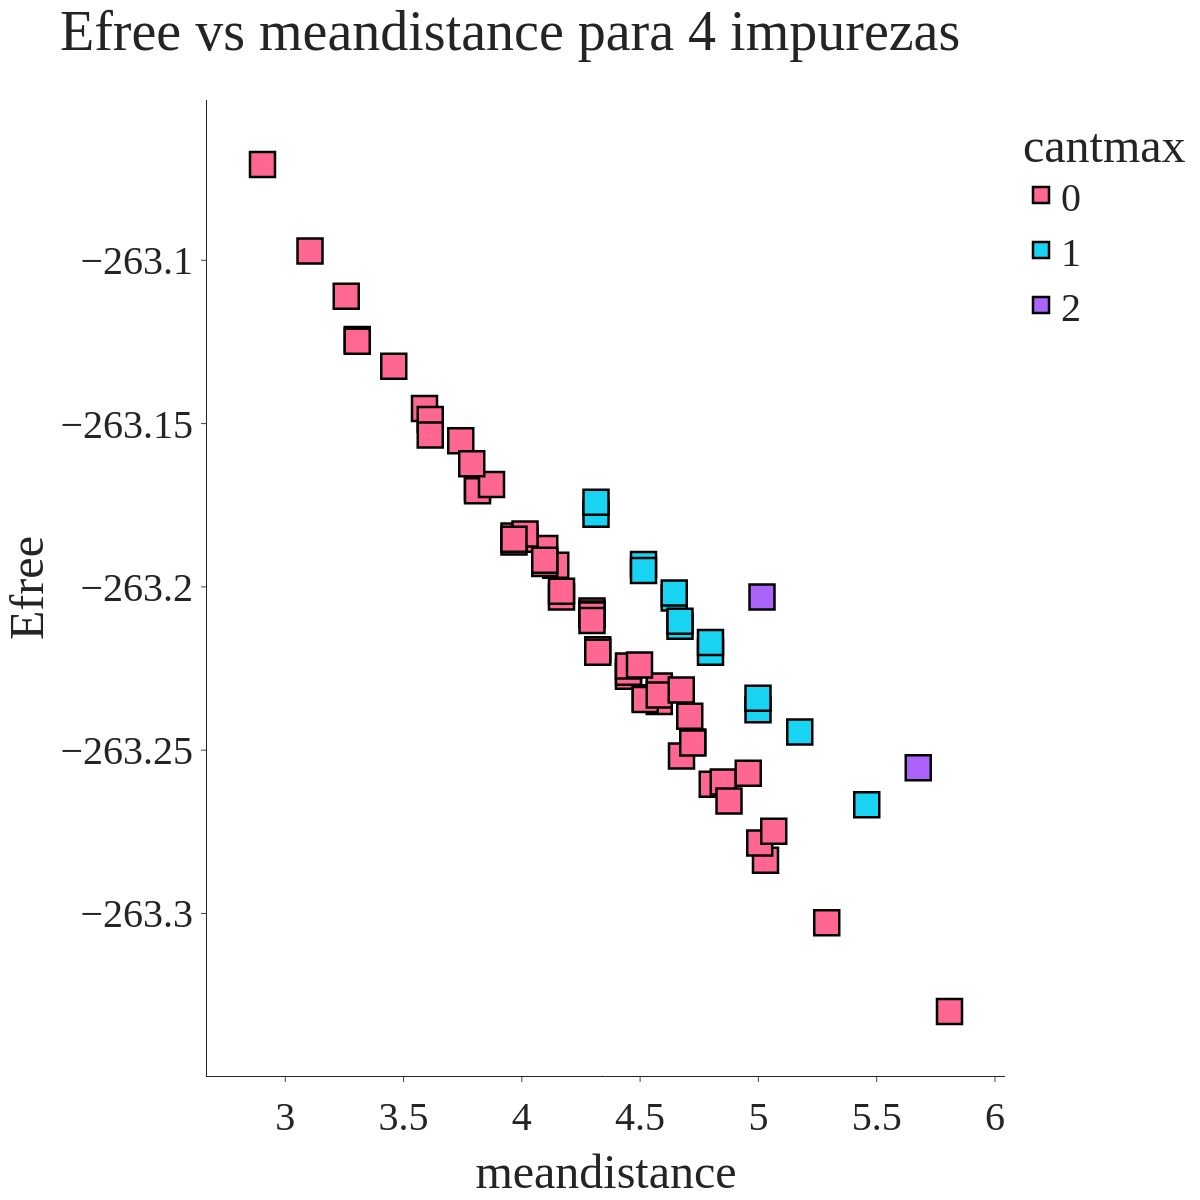
\includegraphics[width=\textwidth]{../code/matrix_multiplication/data/plots/4_impurezas_cantmax_size10.png}
     \end{minipage}%
    \caption{Ejemplo de scatterplot hecho con matplotlib.}
    \label{fig:scatterplot_3}
\end{figure}





\begin{mdframed}
    Recuerde que es imprescindible que se pueda replicar la generación de las gráficas, por lo que usted debe referir a las figuras generadas en `code/matrix\_multiplication/data/plots/` y `code/sorting/data/plots/`.
\end{mdframed}


\newpage
\section{Conclusiones}
\begin{mdframed}
    \textbf{La extensión máxima para esta sección es de 1 página.}
\end{mdframed}

La conclusión de su informe debe enfocarse en el resultado más importante de su trabajo. No se trata de repetir los puntos ya mencionados en el cuerpo del informe, sino de interpretar sus hallazgos desde un nivel más abstracto. En lugar de describir nuevamente lo que hizo, muestre cómo sus resultados responden a la necesidad planteada en la introducción.

\begin{itemize}
    \item  No vuelva a describir lo que ya explicó en el desarrollo del informe. En cambio, interprete sus resultados a un nivel superior, mostrando su relevancia y significado.
    \item Aunque no debe repetir la introducción, la conclusión debe mostrar hasta qué punto logró abordar el problema o necesidad planteada en el inicio. Reflexione sobre el éxito de su análisis o experimento en relación con los objetivos propuestos.
    \item No es necesario restablecer todo lo que hizo (ya lo ha explicado en las secciones anteriores). En su lugar, centre la conclusión en lo que significan sus resultados y cómo contribuyen al entendimiento del problema o tema abordado.
    \item No deben centrarse en sí mismos o en lo que hicieron durante el trabajo (por ejemplo, evitando frases como "primero hicimos esto, luego esto otro...").
    \item Lo más importante es que no se incluyan conclusiones que no se deriven directamente de los resultados obtenidos. Cada afirmación en la conclusión debe estar respaldada por el análisis o los datos presentados. Se debe evitar extraer conclusiones generales o excesivamente amplias que no puedan justificarse con los experimentos realizados.
\end{itemize}


\newpage

\newpage
\appendix


\section{Apéndice 1}
Aquí puede agregar tablas, figuras u otro material que no se incluyó en el cuerpo principal del documento, ya que no constituyen elementos centrales de la tarea. Si desea agregar material adicional que apoye o complemente el análisis realizado, puede hacerlo en esta sección.

\begin{mdframed} 
    Esta sección es solo para material adicional. El contenido aquí no será evaluado directamente, pero puede ser útil si incluye material que será referenciado en el cuerpo del documento. Por lo tanto, asegúrese de que cualquier elemento incluido esté correctamente referenciado y justificado en el informe principal.
 \end{mdframed}


 
\printbibliography

\end{document}


